\documentclass[a4paper,12pt,twoside]{memoir}

% Castellano
\usepackage[spanish,es-tabla]{babel}
\usepackage{graphicx}
\usepackage{float}
\selectlanguage{spanish}
\usepackage[utf8]{inputenc}
\usepackage[T1]{fontenc}
\usepackage{lmodern} % Scalable font
\usepackage{microtype}
\usepackage{placeins}

\usepackage{url}

\RequirePackage{booktabs}
\RequirePackage[table]{xcolor}
\RequirePackage{xtab}
\RequirePackage{multirow}

% Links
\PassOptionsToPackage{hyphens}{url}\usepackage[colorlinks]{hyperref}
\hypersetup{
	allcolors = {red}
}

% Bibliography management
\usepackage[numbers,sort]{natbib}

% Ecuaciones
\usepackage{amsmath}

% Rutas de fichero / paquete
\newcommand{\ruta}[1]{{\sffamily #1}}

% Párrafos
\nonzeroparskip

% Huérfanas y viudas
\widowpenalty100000
\clubpenalty100000

% Imagenes
\usepackage{graphicx}
\newcommand{\imagen}[2]{
	\begin{figure}[!h]
		\centering
		\includegraphics[width=0.9\textwidth]{#1}
		\caption{#2}\label{fig:#1}
	\end{figure}
	\FloatBarrier
}

\newcommand{\imagenflotante}[2]{
	\begin{figure}%[!h]
		\centering
		\includegraphics[width=0.9\textwidth]{#1}
		\caption{#2}\label{fig:#1}
	\end{figure}
}



% El comando \figura nos permite insertar figuras comodamente, y utilizando
% siempre el mismo formato. Los parametros son:
% 1 -> Porcentaje del ancho de página que ocupará la figura (de 0 a 1)
% 2 --> Fichero de la imagen
% 3 --> Texto a pie de imagen
% 4 --> Etiqueta (label) para referencias
% 5 --> Opciones que queramos pasarle al \includegraphics
% 6 --> Opciones de posicionamiento a pasarle a \begin{figure}
\newcommand{\figuraConPosicion}[6]{%
  \setlength{\anchoFloat}{#1\textwidth}%
  \addtolength{\anchoFloat}{-4\fboxsep}%
  \setlength{\anchoFigura}{\anchoFloat}%
  \begin{figure}[#6]
    \begin{center}%
      \Ovalbox{%
        \begin{minipage}{\anchoFloat}%
          \begin{center}%
            \includegraphics[width=\anchoFigura,#5]{#2}%
            \caption{#3}%
            \label{#4}%
          \end{center}%
        \end{minipage}
      }%
    \end{center}%
  \end{figure}%
}

%
% Comando para incluir imágenes en formato apaisado (sin marco).
\newcommand{\figuraApaisadaSinMarco}[5]{%
  \begin{figure}%
    \begin{center}%
    \includegraphics[angle=90,height=#1\textheight,#5]{#2}%
    \caption{#3}%
    \label{#4}%
    \end{center}%
  \end{figure}%
}
% Para las tablas
\newcommand{\otoprule}{\midrule [\heavyrulewidth]}
%
% Nuevo comando para tablas pequeñas (menos de una página).
\newcommand{\tablaSmall}[5]{%
 \begin{table}
  \begin{center}
   \rowcolors {2}{gray!35}{}
   \begin{tabular}{#2}
    \toprule
    #4
    \otoprule
    #5
    \bottomrule
   \end{tabular}
   \caption{#1}
   \label{tabla:#3}
  \end{center}
 \end{table}
}

%
% Nuevo comando para tablas pequeñas (menos de una página).
\newcommand{\tablaSmallSinColores}[5]{%
 \begin{table}[H]
  \begin{center}
   \begin{tabular}{#2}
    \toprule
    #4
    \otoprule
    #5
    \bottomrule
   \end{tabular}
   \caption{#1}
   \label{tabla:#3}
  \end{center}
 \end{table}
}

\newcommand{\tablaApaisadaSmall}[5]{%
\begin{landscape}
  \begin{table}
   \begin{center}
    \rowcolors {2}{gray!35}{}
    \begin{tabular}{#2}
     \toprule
     #4
     \otoprule
     #5
     \bottomrule
    \end{tabular}
    \caption{#1}
    \label{tabla:#3}
   \end{center}
  \end{table}
\end{landscape}
}

%
% Nuevo comando para tablas grandes con cabecera y filas alternas coloreadas en gris.
\newcommand{\tabla}[6]{%
  \begin{center}
    \tablefirsthead{
      \toprule
      #5
      \otoprule
    }
    \tablehead{
      \multicolumn{#3}{l}{\small\sl continúa desde la página anterior}\\
      \toprule
      #5
      \otoprule
    }
    \tabletail{
      \hline
      \multicolumn{#3}{r}{\small\sl continúa en la página siguiente}\\
    }
    \tablelasttail{
      \hline
    }
    \bottomcaption{#1}
    \rowcolors {2}{gray!35}{}
    \begin{xtabular}{#2}
      #6
      \bottomrule
    \end{xtabular}
    \label{tabla:#4}
  \end{center}
}

%
% Nuevo comando para tablas grandes con cabecera.
\newcommand{\tablaSinColores}[6]{%
  \begin{center}
    \tablefirsthead{
      \toprule
      #5
      \otoprule
    }
    \tablehead{
      \multicolumn{#3}{l}{\small\sl continúa desde la página anterior}\\
      \toprule
      #5
      \otoprule
    }
    \tabletail{
      \hline
      \multicolumn{#3}{r}{\small\sl continúa en la página siguiente}\\
    }
    \tablelasttail{
      \hline
    }
    \bottomcaption{#1}
    \begin{xtabular}{#2}
      #6
      \bottomrule
    \end{xtabular}
    \label{tabla:#4}
  \end{center}
}

%
% Nuevo comando para tablas grandes sin cabecera.
\newcommand{\tablaSinCabecera}[5]{%
  \begin{center}
    \tablefirsthead{
      \toprule
    }
    \tablehead{
      \multicolumn{#3}{l}{\small\sl continúa desde la página anterior}\\
      \hline
    }
    \tabletail{
      \hline
      \multicolumn{#3}{r}{\small\sl continúa en la página siguiente}\\
    }
    \tablelasttail{
      \hline
    }
    \bottomcaption{#1}
  \begin{xtabular}{#2}
    #5
   \bottomrule
  \end{xtabular}
  \label{tabla:#4}
  \end{center}
}



\definecolor{cgoLight}{HTML}{EEEEEE}
\definecolor{cgoExtralight}{HTML}{FFFFFF}

%
% Nuevo comando para tablas grandes sin cabecera.
\newcommand{\tablaSinCabeceraConBandas}[5]{%
  \begin{center}
    \tablefirsthead{
      \toprule
    }
    \tablehead{
      \multicolumn{#3}{l}{\small\sl continúa desde la página anterior}\\
      \hline
    }
    \tabletail{
      \hline
      \multicolumn{#3}{r}{\small\sl continúa en la página siguiente}\\
    }
    \tablelasttail{
      \hline
    }
    \bottomcaption{#1}
    \rowcolors[]{1}{cgoExtralight}{cgoLight}

  \begin{xtabular}{#2}
    #5
   \bottomrule
  \end{xtabular}
  \label{tabla:#4}
  \end{center}
}



\graphicspath{ {./img/} }

% Capítulos
\chapterstyle{bianchi}
\newcommand{\capitulo}[2]{
	\setcounter{chapter}{#1}
	\setcounter{section}{0}
	\setcounter{figure}{0}
	\setcounter{table}{0}
	\chapter*{#2}
	\addcontentsline{toc}{chapter}{#2}
	\markboth{#2}{#2}
}

% Apéndices
\renewcommand{\appendixname}{Apéndice}
\renewcommand*\cftappendixname{\appendixname}

\newcommand{\apendice}[1]{
	%\renewcommand{\thechapter}{A}
	\chapter{#1}
}

\renewcommand*\cftappendixname{\appendixname\ }

% Formato de portada
\makeatletter
\usepackage{xcolor}
\newcommand{\tutor}[1]{\def\@tutor{#1}}
\newcommand{\course}[1]{\def\@course{#1}}
\definecolor{cpardoBox}{HTML}{E6E6FF}
\def\maketitle{
  \null
  \thispagestyle{empty}
  % Cabecera ----------------
\noindent
\includegraphics[width=\textwidth]{cabecera}\vspace{1cm}%
  \vfill
  % Título proyecto y escudo informática ----------------
  \colorbox{cpardoBox}{%
    \begin{minipage}{.8\textwidth}
      \vspace{.5cm}\Large
      \begin{center}
      \textbf{TFG del Grado en Ingeniería Informática}\vspace{.6cm}\\
      \textbf{\LARGE\@title{}}
      \end{center}
      \vspace{.2cm}
    \end{minipage}

  }%
  \hfill\begin{minipage}{.20\textwidth}
    
\includegraphics[width=\textwidth]{escudoInfor}
  \end{minipage}
  \vfill
  % Datos de alumno, curso y tutores ------------------
  \begin{center}%
  {%
    \noindent\LARGE
    Presentado por \@author{}\\ 
    en Universidad de Burgos --- \@date{}\\
    Tutores: \@tutor{}\\
  }%
  \end{center}%
  \null
  \cleardoublepage
  }
\makeatother

\newcommand{\nombre}{Alberto Díaz Álvarez} %%% cambio de comando

% Datos de portada
\title{eLearningQA Versión 2\\- Cuestionarios y Foros -}
\author{\nombre}
\tutor{Carlos López Nozal y Raúl Marticorena Sánchez}
\date{\today}

\begin{document}

\maketitle


\newpage\null\thispagestyle{empty}\newpage


%%%%%%%%%%%%%%%%%%%%%%%%%%%%%%%%%%%%%%%%%%%%%%%%%%%%%%%%%%%%%%%%%%%%%%%%%%%%%%%%%%%%%%%%
\thispagestyle{empty}


\noindent
\includegraphics[width=\textwidth]{cabecera}\vspace{1cm}

\noindent D. Raúl Marticorena Sánchez, profesor del departamento de Ingeniería Informática,
área de Lenguajes y Sistemas Informáticos.

\noindent D. Carlos López Nozal, profesor del departamento de Ingeniería Informática,
área de Lenguajes y Sistemas Informáticos.

\noindent Exponen:

\noindent Que el alumno D. \nombre, con DNI 03929601M, ha realizado el Trabajo final de Grado en Ingeniería Informática titulado \textit{eLearningQA - Control de calidad}. 

\noindent Y que dicho trabajo ha sido realizado por el alumno bajo la dirección del que suscribe, en virtud de lo cual se autoriza su presentación y defensa.

\begin{center} %\large
En Burgos, {\large \today}
\end{center}

\vfill\vfill\vfill

% Author and supervisor
\begin{minipage}{0.45\textwidth}
\begin{flushleft} %\large
Vº. Bº. del Tutor:\\[2cm]
D. Raúl Marticorena Sánchez
\end{flushleft}
\end{minipage}
\hfill
\begin{minipage}{0.45\textwidth}
\begin{flushleft} %\large
Vº. Bº. del tutor:\\[2cm]
D. Carlos López Nozal
\end{flushleft}
\end{minipage}
\hfill

\vfill

% para casos con solo un tutor comentar lo anterior
% y descomentar lo siguiente
%Vº. Bº. del Tutor:\\[2cm]
%D. nombre tutor


\newpage\null\thispagestyle{empty}\newpage




\frontmatter

% Abstract en castellano
\renewcommand*\abstractname{Resumen}
\begin{abstract}
Este Trabajo de Fin de Grado se centra en la mejora de un proyecto existente que se enfoca en el control de calidad de los cursos asignados a un profesor. En esta implementación, se busca la mejora continua del proyecto al especializarse en la optimización de los cuestionarios y foros presentes en los cursos impartidos por dicho profesor. Al revisar a primera vista esta nueva versión, será posible comprender la estructura del curso, identificar los principales fallos y analizar la forma en que los alumnos interactúan con dichos recursos. Es crucial que el profesor comprenda la participación de los estudiantes para poder adaptar los recursos y mantener un alto nivel de participación y atención.
En resumen, esta versión mejorada del proyecto tiene como objetivo principal maximizar la participación y atención de los estudiantes a través de una especialización de los cuestionarios y foros. Al comprender la dinámica de la clase y adaptar los recursos de manera adecuada, se espera alcanzar un mayor nivel de calidad en la experiencia de aprendizaje y promover un ambiente enriquecedor para todos los involucrados.
\end{abstract}

\renewcommand*\abstractname{Descriptores}
\begin{abstract}
Aplicación web, framework de calidad en e-learning, revisiones automáticas, calidad en cursos en línea, Learning Management System (LMS).
\end{abstract}

\clearpage

% Indices
\tableofcontents

\clearpage

\listoffigures

\clearpage

\listoftables
\clearpage

\mainmatter
\capitulo{1}{Introducción}

En el presente Trabajo de Fin de Grado (TFG), se aborda el desarrollo de una aplicación innovadora que se centra en el aseguramiento de la calidad en el ámbito del e-learning. El e-learning, o aprendizaje electrónico, ha experimentado un crecimiento significativo en los últimos años. Hoy, la distancia ya no es un obstáculo en la educación; no es necesario asistir a las aulas, sino que desde nuestro lugar podemos acceder a la formación académica a través de la educación virtual\cite{educacionvirtual2023}.

Sin embargo, a medida que el e-learning se ha expandido, también han surgido desafíos en términos de asegurar la calidad de los contenidos y las experiencias de aprendizaje ofrecidas. Es fundamental garantizar que los recursos educativos en línea sean efectivos, accesibles, relevantes y estén diseñados de acuerdo con los estándares y las mejores prácticas establecidas\cite{buenaspracticas2017}.

El objetivo principal de esta aplicación web es proporcionar a los usuarios un resumen general de cómo está planteado el curso y la viabilidad del mismo. Esta segunda versión busca un nivel de detalle más profundo en el que se intenta mostrar al usuario un conjunto de estadísticas respecto a los cuestionarios y foros dejando al descubierto el interés del alumnado por dicha asignatura. Dichas estadísticas se podrán interpretar de la forma que el usuario vea conveniente. 

La aplicación permitirá a los usuarios realizar evaluaciones sistemáticas de los cursos en línea, identificando fortalezas y áreas de mejora en cada aspecto relevante. Además, ofrecerá una vista de los principales fallos para mejorar la calidad de los cursos, ayudando a los profesionales del e-learning a desarrollar experiencias de aprendizaje mejor adaptadas al marco de calidad.

A lo largo de este trabajo, se describirá en detalle el proceso de desarrollo de la aplicación, desde el diseño de la arquitectura y la interfaz de usuario, hasta la implementación de las funcionalidades clave. Se abordarán los desafíos técnicos y las decisiones de diseño tomadas, así como las pruebas y validaciones realizadas para garantizar el correcto funcionamiento de la aplicación.

Además, se explorarán y analizarán las normativas, estándares y mejores prácticas relevantes en el ámbito del aseguramiento de la calidad en el e-learning, con el fin de fundamentar y respaldar las funcionalidades proporcionadas por la aplicación.
\capitulo{2}{Objetivos del proyecto}

El objetivo principal de este trabajo es desarrollar una aplicación web que permita al profesor evaluar las distintas fases de diseño instruccional de un curso de Moodle (diseño, implementación, realización, evaluación), tal como recomiendan algunos frameworks internacionales de calidad en e-learning \cite{previotfg}.

Como objetivos añadidos al trabajo previo se ha decidido profundizar en el apartado de los cuestionarios y los foros intentando conseguir un informe detallado en esos áreas. Consiguiendo así una rápida lectura de la viabilidad del curso con la posibilidad de obtener detalles en las posibes zonas de mejora.

A continuación detallaré los subojetivos que darán pie al cumplimiento del objetivo principal:
\begin{enumerate}
    \item Definir los modelos y sus respectivos atributos de los cuestionarios, intentos y foros.
    \item Aprender a combinar los servicios Web de Moodle para adaptar sus respuestas a los datos que queremos mostrar en la aplicación.
    \item Aplicar los frameworks internacionales de calidad en e-learning a los datos que reproducirá el proyecto.
    \item Diseñar indicadores cualitativos y cuantitativos de calidad de cada fase de diseño instruccional del curso en línea (diseño, implementación, realización y evaluación)\cite{previotfg}
\end{enumerate}
\capitulo{3}{Conceptos teóricos}


\section{Definiciones básicas}

\begin{itemize}
	\item \textbf{Administración de la calidad:} es el conjunto de actividades para definir un proceso de mejora continua: aseguramiento de calidad, planeación de calidad y control de calidad \cite{dolado2000medicion} \cite{Sommerville10}.
	\item \textbf{Aseguramiento de calidad:} establecimiento de un marco de trabajo de procedimientos y estándares que conducen a un curso de alta calidad.
	\item \textbf{Planeación de calidad:} selección de procedimientos y estándares del
	marco de trabajo y adaptación para un curso concreto del software específico.
	\item \textbf{Control de calidad:} los estándares y procedimientos seguidos por el
	equipo de desarrollo.
	
	\item \textbf{Medición:} el proceso por el cuál se asignan números o símbolos a los atributos de las entidades del
	curso en línea, de tal forma que los caracteriza de manera clara a través de reglas o consultas sobre LMS.
	
	\item \textbf{E-learning:}
	es el proceso de enseñanza y aprendizaje impartido por medios electrónicos como internet, plataformas virtuales, medios audiovisuales, etc.
	\item \textbf{LMS:}
	Learning Management Systems, o sistemas de gestión del aprendizaje son plataformas online que permiten gestionar el aprendizaje de grupos de personas en un entorno virtual. El aprendizaje en este tipo de plataformas no se limita al campo académico, sino que también se pueden usar los LMS dentro de empresas para instruir a los empleados. Entre los más populares se encuentran Moodle, Edmodo y Blackboard.
	\item \textbf{Moodle:}
	es una plataforma de aprendizaje LMS que permite a los profesores crear entornos de aprendizaje altamente personalizables. Fue creado por Martin Dougiamas que publicó su primera versión el 20 de agosto de 2002 \cite{dougiamas2002interpretive}.
\end{itemize}


\section{Marco de referencia de calidad de MOOQ}
La calidad se puede definir como la capacidad de satisfacer una serie de necesidades y en el caso del e-learning se trata de las necesidades educativas del alumno, como la calidad del material educativo o la ayuda a la comprensión de este.

Ahora pasamos a explicar las tres dimensiones del marco de referencia de calidad en e-learning de MOOQ \cite{stracke2018quality}. MOOQ es la alianza europea por la calidad de los MOOC (Massive Open Online Courses). Un MOOC varía respecto al caso de e-learning para el que pretendemos crear la aplicación, pero al reducir la calidad del diseño instruccional a sus fases, roles y perspectivas aplicado a un tipo de e-learning es lo suficientemente válido.

En esta segunda versión los cambios que se han implementado se encuentran en la fase de diseño y realización, pero se mantendrá el resto del información para comprender todo el proyecto.

\subsection{Fases}
\begin{itemize}
	\item \textbf{Análisis:}
	En esta fase se definen los objetivos, el contexto, y los recursos (docentes, tiempo, presupuesto...) para la ejecución para comprender la situación inicial.
	\item \textbf{Diseño:}
	En esta fase se define lo que se planea hacer a partir de los resultados de la fase de análisis, como por ejemplo el enfoque de enseñanza que se piensa llevar a cabo: diseños asistidos por el profesor basados en comunicaciones síncronas o asíncronas, diseños sin supervisión del profesor basados en recursos y actividades de aprendizajes, o mixtos.
	\item \textbf{Implementación:}
	En esta fase se define de qué manera se van a llevar a cabo los planes descritos en la fase de diseño, como por ejemplo de qué manera se va a producir el contenido.
	\item \textbf{Realización:}
	Esta fase es en la que se interactúa con el alumno, se gestionan los problemas técnicos y las dudas de los alumnos, además de evaluar su aprendizaje.
	\item \textbf{Evaluación:}
	En esta última fase se evalúa la calidad del resto de fases mediante encuestas, entrevistas, u otros medios.
\end{itemize}

\imagen{CicloFases.png}{Ciclo de fases según el marco de MOOQ \cite{stracke2018quality}}

\subsection{Roles}
Los roles son conjuntos de responsabilidades asumidos por una o más personas. Una persona podría tomar dos o más roles dado el caso (diseñador y facilitador, por ejemplo).
\begin{itemize}
	\item \textbf{Diseñadores:}
	Los encargados de decidir de qué forma se van a impartir el curso y generan el contenido (autores, expertos en el tema, diseñadores instruccionales).
	\item \textbf{Facilitadores:}
	Son aquellos que conocen la materia a enseñar y son capaces de explicarlo y dar feedback, además de seguir el aprendizaje de los alumnos.
	\item \textbf{Proveedores:}
	Son los encargados de proveer los medios digitales para llevar a cabo el e-learning (programadores, diseñadores y desarrolladores de software).
\end{itemize}


\subsection{Perspectivas}
\begin{itemize}
	\item \textbf{Pedagógica:}
	El punto de vista que se centra en el contenido y en el aprendizaje por parte del alumno. Los procesos relacionados tienen que ver con el contenido, el feedback, y la evaluación de los alumnos.
	\item \textbf{Tecnológica:}
	El punto de vista que se centra en las necesidades tecnológicas del curso. La mayoría de los procesos está relacionada con esta perspectiva debido a la naturaleza del e-learning.
	\item \textbf{Estratégica:}
	El punto de vista que se centra en la consecución de los objetivos del curso dentro del tiempo y presupuesto establecidos para este. Los procesos relacionados tienen que ver con los objetivos, conceptos y el contexto en el que se enseña (presupuesto, demanda, competencia...).
\end{itemize}

\section{Buenas prácticas de la docencia online}
A continuación presentamos una serie de buenas prácticas que la aplicación pretende fomentar. También nos basamos en la experiencia que se ha tenido como alumno en la plataforma UBUVirtual. Estas cuestiones no llegan a cubrir por completo lo que sería una especie de guía para gestionar cursos virtuales, es un complemento al framework de calidad.
\subsection{Retroalimentación a tiempo}
Es importante que el docente responda a las dudas a tiempo, y también que el alumno conozca sus resultados en un tiempo razonable, y esto es por dos razones: la primera, que el alumno no pierda la motivación si tiene buenos resultados, y la segunda, que se esfuerce más si tiene resultados mejorables.
\subsection{Tener en cuenta la opinión de los alumnos}
La evaluación es una parte fundamental del ciclo del diseño instruccional.
Las encuestas permiten encontrar los puntos fuertes (para no alterarlos) y los débiles (para solventarlos).

\subsection{Revisar los cuestionarios}
Es muy útil tener en cuenta las estadísticas de los cuestionarios, aunque, son necesarios suficientes intentos por parte de los estudiantes para tener una validez razonable. Una de esas estadísticas es el índice de facilidad, que indica el porcentaje medio de la puntuación que obtienen los alumnos de una pregunta, indicando su dificultad. Otra estadística interesante es la calificación aleatoria estimada, que expresa el resultado medio de responder aleatoriamente una pregunta de tipo test; en un caso ideal este valor sería de 0\%, si no, la puntuación de esa pregunta tendría un componente aleatorio. Por último, la eficiencia discriminativa\cite{discrimination-2021} indica como de buena es una pregunta discriminando entre alumnos que saquen buena nota en el cuestionario y aquellos que saquen peor nota. Hay que tener en cuenta estos valores para conseguir cuestionarios más justos y efectivos.

También es importante que las preguntas tengan una retroalimentación asignada para que los alumnos aprendan del resultado en la revisión.

Es recomendable ajustar el tiempo que se permite para la realización de los cuestionarios a partir del tiempo que tomó realizarlo en anteriores ocasiones para dificultar el fraude y tampoco quedarse corto y no dejar a los alumnos terminar.

\subsection{Trabajo en equipo}
Obtener las competencias necesarias para el trabajo en equipo es fundamental para el alumno, sobretodo en la universidad, que pretende preparar a sus estudiantes para un entorno laboral. Es muy recomendable que un curso contenga actividades con entrega por grupos.

\subsection{Claridad y corrección}
La corrección y la claridad de la información en un curso ayuda a evitar que el alumno se pierda en las formas y entienda mejor lo que se pide de él.
El calificador debería mostrar de forma concisa el peso de cada procedimiento, no tener demasiadas categorías dentro de otras y si las notas máximas de cada actividad coinciden, leer los resultados se vuelve mucho más sencillo.

\subsection{Apuntes actualizados}
Aparte de que viene bien revisar los materiales proporcionados a los alumnos en busca de errores y para añadir novedades, el no hacerlo en mucho tiempo da al alumno una imagen de abandono por parte del profesor, y en mi experiencia como alumno he llegado a vivir esa situación.

\subsection{Diferentes formas de interactuar en el curso}
Es muy importante abrir al alumno varias vías para interactuar con un curso específico como pueden ser los foros, tutorías o cuestionarios ya que permiten al alumno sentir cierto dinamismo durante los meses que se encuentre estudiando dicha asignatura o módulo. Esto permite pensar al alumno durante ciertos momentos que se encuentra dentro de un aula dejando de lado la distancia que implica el e-Learning.

\subsection{Conocer la participación}
Conocer la participación en sectores como los foros puede ayudar a comprender si los alumnos se encuentra motivados en la asignatura o en un tema o si por el contrario es necesario buscar alguna forma de fomentar dicha participación.

\section{Plan de calidad para cursos e-learning}
En secciones previas hemos presentado un marco de calidad genérico junto con recomendaciones del Centro de Enseñanza Virtual de la Universidad de Burgos junto a la identificación de unas buenas prácticas de enseñanza en cursos en línea.

A partir de esta documentación en este sección definimos de manera concreta unos indicadores cualitativos y cuantitativos de calidad basados en consultas a entidades de cursos en línea.

Para facilitar la comprensión del conjunto de consultas de calidad se agrupan en las fases del marco de referencia de calidad de MOOQ \cite{stracke2018quality}. La Tabla \ref{table:diseño} muestra el  conjunto  de consultas de  fase de diseño, la Tabla \ref{table:implementación} las de la fase de implementación, la Tabla \ref{table:realización} las de la fase de realización y la Tabla \ref{table:evaluación} las de la fase de evaluación.
En este apartado definiremos qué información intentamos conseguir de cada fase (nos vamos a centrar en las fases de diseño, implementación, realización, y evaluación), rol y perspectiva mediante distintos métodos. La mayoría de consultas provienen de la lista de comprobación del Centro de Enseñanza Virtual de la Universidad de Burgos (UBUCEV) de asignaturas virtuales.
Los procesos indicados en la última columna de las tablas se refieren a los procesos que se indican a partir de la página 10 del documento del marco de referencia de calidad de MOOC \cite{stracke2018quality}. \\
\\
Los cambios introducidos en la versión 2 del proyecto se incluirán en azul para distinguirlos en las tablas. Es importante concocer de un vistazo cuáles son las nuevas funcionalidades o conceptos para ser conscientes del crecimiento del proyecto con sus distintas versiones.

\label{consultas}
\begin{table}[H]
\caption{Consultas de diseño \linebreak Leyenda:
	\linebreak Responsabilidad: R=Responsable,X=Involucrado
	\linebreak Perspectivas: P=Pedagógica, T=Tecnológica, E=Estratégica}\label{table:diseño}
\resizebox{\textwidth}{!}{%
	\begin{tabular}{|l|l|l|l|l|l|}
		\hline
		\textbf{Consulta}                                                                                                                             & \textbf{Perspectivas} & \textbf{Diseñador} & \textbf{Facilitador} & \textbf{Proveedor} & \textbf{Proceso} \\ \hline
		\begin{tabular}[c]{@{}l@{}}Las opciones\\ de progreso\\ del estudiante\\ están activadas\end{tabular}                                & P            & R         & X           &           & D-5     \\ \hline
		\begin{tabular}[c]{@{}l@{}}Se proporcionan\\ contenidos en\\ diferentes formatos\end{tabular}                                        & PT           & R         & X           & X         & D-4     \\ \hline
		\begin{tabular}[c]{@{}l@{}}El curso tiene\\ grupos\end{tabular}                                                                      & P            & R         & X           & X         & D-3     \\ \hline
		\begin{tabular}[c]{@{}l@{}}El curso tiene\\ actividades\\ grupales\end{tabular}                                                      & P            & R         & X           & X         & D-3     \\ \hline
		\begin{tabular}[c]{@{}l@{}}\textcolor{blue}{El curso tiene}\\ \textcolor{blue}{cuestionarios}\end{tabular}                                                      & \textcolor{blue}{P}            & \textcolor{blue}{R}         & \textcolor{blue}{X}           & \textcolor{blue}{X}         &      \\ \hline
		\begin{tabular}[c]{@{}l@{}}\textcolor{blue}{El curso tiene}\\ \textcolor{blue}{foros}\end{tabular}                                                      & \textcolor{blue}{P}            & \textcolor{blue}{R}         & \textcolor{blue}{X}           & \textcolor{blue}{X}         &      \\ \hline
		\begin{tabular}[c]{@{}l@{}}Los estudiantes\\ pueden ver las\\ condiciones\\ necesarias para\\ completar una\\ actividad\end{tabular} & P            & R         & X           & X         &      \\ \hline
		\begin{tabular}[c]{@{}l@{}}Todas las\\ actividades tienen\\ la misma nota\\ máxima en el\\ calificador\end{tabular}                  & P            & R         & X           & X         &      \\ \hline
		\begin{tabular}[c]{@{}l@{}}Las preguntas de\\ los cuestionarios\\ tienen\\ retroalimentación\end{tabular}                                        & P           & R         & X           & X         &      \\ \hline
		\begin{tabular}[c]{@{}l@{}}Las preguntas de\\ opción multiple\\ puntúan con una\\ calificación aleatoria\\ estimada de cero\end{tabular}                                        & P           & R         & X           & X         &      \\ \hline
	\end{tabular}%
}
\end{table}

\begin{table}[H]
\caption{Consultas de implementación \linebreak Leyenda:
	\linebreak Responsabilidad: R=Responsable,X=Involucrado
	\linebreak Perspectivas: P=Pedagógica, T=Tecnológica, E=Estratégica}\label{table:implementación}
\resizebox{\textwidth}{!}{%
	\begin{tabular}{|l|l|l|l|l|l|}
		\hline
		\textbf{Consulta}                                                                                                                             & \textbf{Perspectivas} & \textbf{Diseñador} & \textbf{Facilitador} & \textbf{Proveedor} & \textbf{Proceso} \\ \hline
		\begin{tabular}[c]{@{}l@{}}Los recursos\\ están actualizados\end{tabular}                                  & PT           & R         & X           & X         & I-1     \\ \hline
		\begin{tabular}[c]{@{}l@{}}Fechas de apertura\\ y cierre de tareas\\ son correctas\end{tabular}            & PT           & X         & R           & X         & R-2     \\ \hline
		\begin{tabular}[c]{@{}l@{}}Se detallan los\\ criterios de\\ evaluación\\ (rúbricas, ejemplos)\end{tabular} & PT           & R         & X           & X         & R-3     \\ \hline
		\begin{tabular}[c]{@{}l@{}}El calificador no\\ tiene demasiado\\ anidamiento\end{tabular} & PE           & R         & X           & X         &      \\ \hline
		\begin{tabular}[c]{@{}l@{}}Los alumnos\\ están divididos\\ en grupos\end{tabular}                          & TE           & X         &             & R         & I-6     \\ \hline
	\end{tabular}%
}
\end{table}


\begin{table}[H]
\caption{Consultas de realización \linebreak Leyenda:
	\linebreak Responsabilidad: R=Responsable,X=Involucrado
	\linebreak Perspectivas: P=Pedagógica, T=Tecnológica, E=Estratégica}\label{table:realización}
\resizebox{\textwidth}{!}{%
	\begin{tabular}{|l|l|l|l|l|l|}
		\hline
		\textbf{Consulta}                                                                                                                             & \textbf{Perspectivas} & \textbf{Diseñador} & \textbf{Facilitador} & \textbf{Proveedor} & \textbf{Proceso} \\ \hline
		\begin{tabular}[c]{@{}l@{}}El profesor\\ responde en los\\ foros dentro del\\ límite de 48 horas\\ lectivas desde que\\ se plantea la duda\end{tabular} & PT           & X         & R           & X         & R-2     \\ \hline
		\begin{tabular}[c]{@{}l@{}}Se ofrece\\ retroalimentación\\ de las tareas\end{tabular}                                                                   & PT           & X         & R           & X         & R-2     \\ \hline
		\begin{tabular}[c]{@{}l@{}}Las tareas están\\ calificadas\end{tabular}                                                                                  & PT           & X         & R           & X         & R-2     \\ \hline
		\begin{tabular}[c]{@{}l@{}}El calificador\\ muestra cómo\\ ponderan las\\ diferentes tareas\end{tabular}                                                & PT           & X         & R           & X         & R-2     \\ \hline
		\begin{tabular}[c]{@{}l@{}}El tiempo de\\ los cuestionarios\\ está bien ajustado\end{tabular}                                        & P           & R         & X           & X         &      \\ \hline
		\begin{tabular}[c]{@{}l@{}}Los cuestionarios\\ tienen una dificultad\\ estimada entre unos \\valores umbrales\end{tabular}                                        & P           & R         & X           & X         &      \\ \hline
		\begin{tabular}[c]{@{}l@{}}Las preguntas de\\ los cuestionarios\\ son buenas\\ discriminando\cite{discrimination-2021}\end{tabular}                                        & P           & R         & X           & X         &      \\ \hline
		\begin{tabular}[c]{@{}l@{}}\textcolor{blue}{Un porcentaje}\\ \textcolor{blue}{establecido de}\\ \textcolor{blue}{alumnos participa}\\ \textcolor{blue}{en los cuestionarios}\end{tabular}                                                      & \textcolor{blue}{P}            & \textcolor{blue}{X}         & \textcolor{blue}{X}           & \textcolor{blue}{R}         &      \\ \hline
		\begin{tabular}[c]{@{}l@{}}\textcolor{blue}{Un porcentaje}\\ \textcolor{blue}{establecido de}\\ \textcolor{blue}{alumnos participa}\\ \textcolor{blue}{en los foros}\end{tabular}                                                      & \textcolor{blue}{P}            & \textcolor{blue}{X}         & \textcolor{blue}{X}           & \textcolor{blue}{R}         &      \\ \hline
	\end{tabular}%
}
\end{table}

\begin{table}[H]
\caption{Consultas de evaluación \linebreak Leyenda:
	\linebreak Responsabilidad: R=Responsable,X=Involucrado
	\linebreak Perspectivas: P=Pedagógica, T=Tecnológica, E=Estratégica}\label{table:evaluación}
\resizebox{\textwidth}{!}{%
	\begin{tabular}{|l|l|l|l|l|l|}
		\hline
		\textbf{Consulta}                                                                                                                             & \textbf{Perspectivas} & \textbf{Diseñador} & \textbf{Facilitador} & \textbf{Proveedor} & \textbf{Proceso} \\ \hline
		\begin{tabular}[c]{@{}l@{}}La mayoría de\\ alumnos responden\\ a los feedbacks\end{tabular} & PTE          & X         & X           & R         & E-2     \\ \hline
		\begin{tabular}[c]{@{}l@{}}Se utilizan encuestas\\ de opinión\end{tabular}                  & PTE          & X         & X           & R         & E-2     \\ \hline
	\end{tabular}%
}
\end{table}


\capitulo{4}{Técnicas y herramientas}
\section{Desarrollo ágil}
Durante la realización de esta segunda versión se ha mantenido la metodogía de desarrollo ágil siguiendo la línea de una evolución constante, permitiendo la obtención del feedback entre alumno y tutores de forma continua.
\subsection{Desarrollo iterativo}
El desarrollo consiste en la revisión cíclica sobre un mismo trabajo. En este caso se han realizado sprints de entre 7 y 14 días en los que se establecía una reunión en la plataforma Microsoft Teams al final del sprint mostrando los resultados y recibiendo una retroalimentación de los errores, posibles mejoras y características interesantes de implementar de cara al siguiente sprint. A partir del décimo sprint buscando una mejor comprensión del trabajo realizado se ha decidido incorporar el uso de milestones en GitHub.
\subsection{Desarrollo incremental}
El desarrollo incremental sigue la dinámica del desarrollo iterativo buscando la continua mejora gracias al feedback obtenido. Con este procedimiento se han ido realizando varias release a lo largo del trabajo. Una release es una nueva versión del sistema que se está desarrollando \cite{releasedefinition}.
\subsection{Control de versiones}
El control de versiones es un sistema que se utiliza para gestionar y controlar los cambios realizados en los archivos y documentos de un proyecto o sistema de software a lo largo del tiempo. Permite realizar un seguimiento de las modificaciones, controlar quién ha realizado cada cambio, revertir a versiones anteriores y colaborar de manera efectiva en el desarrollo de software.

El control de versiones es especialmente importante en el desarrollo de software, donde múltiples personas trabajan en el mismo proyecto y realizan cambios en los archivos de código fuente. Con un sistema de control de versiones, los desarrolladores pueden guardar y compartir las versiones de su código, fusionar los cambios realizados por diferentes personas y resolver conflictos que puedan surgir \cite{ZOLKIFLI2018408}.
\subsection{GitHub}
GitHub es una plataforma web de alojamiento y colaboración para proyectos de desarrollo de software que utiliza un sistema de control de versiones distribuido llamado Git. En este proyecto, GitHub ha sido utilizado como plataforma de alojamiento para almacenar y compartir el código fuente.

Una de las funcionalidades clave de GitHub es la capacidad de realizar \textit{push} de cambios a un repositorio. El \textit{push} es el acto de enviar los cambios locales a un repositorio remoto en GitHub. Esto permite a los desarrolladores compartir su código y colaborar con otros miembros del equipo de desarrollo \cite{10.1145/2675133.2675284}.
\subsection{Extensión de Visual Studio Code - Git Graph}
Git Graph es una extensión del editor de texto Visual Studio Code que proporciona una interfaz gráfica interactiva para visualizar y navegar por la historia de un repositorio de Git. Permite a los desarrolladores ver de manera intuitiva el historial de cambios, las ramas, las fusiones y las etiquetas de un proyecto Git.

Esta extensión muestra un gráfico visual en forma de árbol que representa la estructura del historial de commits del repositorio. Cada commit se muestra como un nodo en el gráfico y las líneas conectan los nodos para mostrar la relación entre ellos. Además, Git Graph proporciona información adicional sobre cada commit, como el autor, el mensaje de commit y la fecha, como se puede ver en la figura \ref{img:gitgraph}. 
\begin{figure}
  \centering
  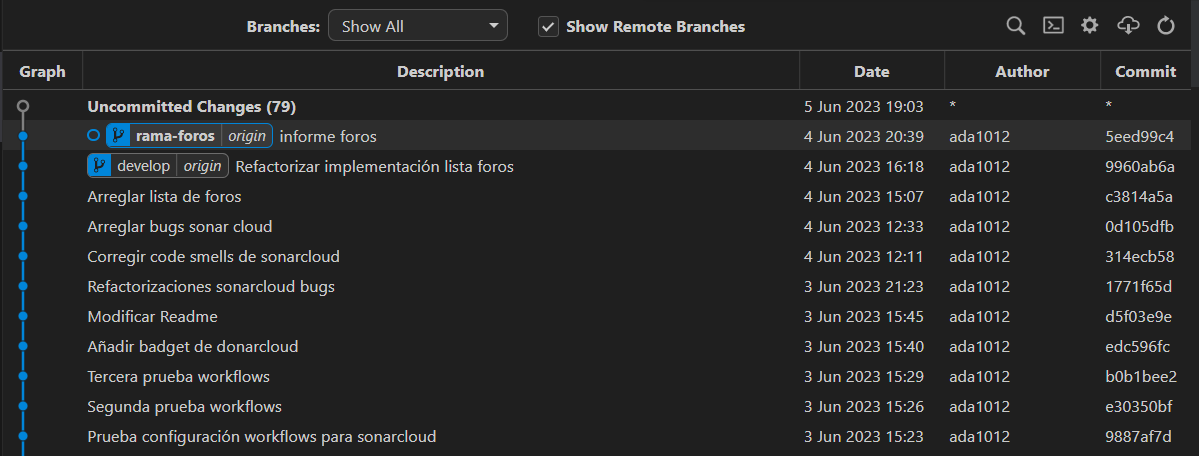
\includegraphics[width=1\textwidth]{GitGraph.png}
  \caption{Extensión de Visual Studio Code - Git Graph}
  \label{img:gitgraph}
\end{figure}
\subsection{Postman}
Es una aplicación que facilita el proceso de desarrollo, prueba y documentación de API (Interfaces de Programación de Aplicaciones). Proporciona una interfaz intuitiva y amigable que permite a los desarrolladores realizar solicitudes HTTP a servidores web y recibir respuestas en tiempo real. Con Postman, los usuarios pueden enviar diferentes tipos de solicitudes, como GET, POST, PUT y DELETE, así como configurar encabezados, parámetros y cuerpos de solicitud personalizados \cite{Christudas2019}.
\subsection{Publicaciones frecuentes}
Una publicación o release consiste en desplegar una aplicación funcional que permite la interacción de los usuarios con dicho producto. Durante el desarrollo del proyecto se han publicado 3 versiones.
\subsection{Refactorización}
La refactorización es el proceso de modificar el diseño interno de un código fuente sin cambiar su comportamiento externo. Se trata de mejorar la estructura y la calidad del código sin añadir nuevas funcionalidades o alterar su funcionalidad existente. El objetivo principal de la refactorización es hacer que el código sea más legible, mantenible y eficiente \cite{asse2015}. En este proyecto se ha implementado SonarCloud para detectar los fallos (\textit{bugs, code smells, vulnerabilities}) y posteriormente realizar dichas refactorizaciones .
\subsection{Uso de test unitarios}
Un test unitario es una técnica de pruebas en el desarrollo de software que tiene como objetivo verificar el correcto funcionamiento de una unidad de código, por lo general, una función, método o clase, de forma aislada e independiente del resto del sistema. En esta aplicación se ha utilizado JUnit para el desarrollo y posterior ejecución de los test \cite{8823472}.
\subsubsection{JUnit}
JUnit es un framework de pruebas unitarias en Java que proporciona un entorno para escribir, organizar y ejecutar pruebas de manera automatizada. Es ampliamente utilizado en el desarrollo de software para garantizar la calidad y funcionalidad de los componentes individuales del código \cite{8823472}.
\subsection{Construcción automática}
La construcción automática se refiere al proceso de utilizar herramientas especializadas, como Maven o Gradle, para automatizar tareas como la compilación del código fuente, la ejecución de pruebas y la generación de archivos de distribución del software. Estas herramientas permiten simplificar y agilizar el proceso de construcción del software, garantizando la consistencia y facilitando su integración en los flujos de trabajo de desarrollo.
\subsubsection{Maven}
Maven es una herramienta de gestión de proyectos de software ampliamente utilizada en el ecosistema de desarrollo de Java. Proporciona un enfoque estructurado y basado en convenciones para la construcción, gestión de dependencias y generación de proyectos. Maven simplifica la configuración y automatiza tareas comunes, como la compilación, la ejecución de pruebas, la generación de informes y la creación de distribuciones del software \cite{packt2014}.
\subsection{Integración continua}
La integración continua es una práctica de desarrollo de software en la que los cambios de código se integran y se prueban automáticamente de forma regular. Consiste en utilizar herramientas y sistemas de automatización para compilar, probar y validar el código constantemente. Esto permite detectar y solucionar errores de manera temprana, facilitando la entrega de software de calidad de forma rápida y frecuente. 
El proyecto contiene un archivo \texttt{yml} que especifica las acciones a seguir para la construcción automática del proyecto y el análisis de calidad de SonarCloud tras cada \textit{push} a la rama \textit{develop} del repositorio.
\subsection{Herramienta de calidad de código: SonarCloud}
SonarCloud es una plataforma en la nube que ofrece servicios de análisis estático de código para evaluar la calidad del software. Proporciona un conjunto de herramientas y métricas que permiten identificar problemas de código, vulnerabilidades, duplicaciones y otras deficiencias en el código fuente. SonarCloud realiza un análisis exhaustivo y genera informes detallados sobre la calidad y la salud general del proyecto. Ayuda a los equipos de desarrollo a mejorar la mantenibilidad, la eficiencia y la seguridad del software mediante la identificación temprana de posibles problemas y la adopción de buenas prácticas de programación.
En este proyecto se integra con los \textit{actions} de GitHub para analizar el proyecto a la hora de realizar un push en la rama develop.
Se puede ver la evolución de la calidad del código en \url{https://sonarcloud.io/project/activity?category=QUALITY_GATE&id=ada1012_eLearningQA}.

\section{Herramientas de desarrollo}
\subsection{Entorno de desarrollo integrado: Eclipse y Visual Studio Code}
Por motivos personales en este trabajo se han utilizado dos entornos de desarrollo, Eclipse y Visual Studio Code. Esta decisión se ha tomado por la comodidad de configuración de archivos de Eclipse y la interfaz amigable de Visual Studio Code. Este último permite instalar varias extensiones como Git Graph o GitHub Copilot que hacen la programación mucho más amena.
\subsection{Extensión de Visual Studio Code - GitHub Copilot}
GitHub Copilot es una herramienta desarrollada por GitHub y OpenAI que utiliza inteligencia artificial (IA) para proporcionar sugerencias y autocompletar código mientras se escribe en diferentes lenguajes de programación. Funciona como una extensión para el editor de código y aprovecha los modelos de lenguaje generativos de OpenAI, como GPT-3, para ofrecer recomendaciones de código en tiempo real.
Esto permite obtener recomendaciones de código sin necesidad de acudir al navegador.
\subsection{Framework CSS: Bootstrap}
Bootstrap es un framework CSS de código abierto ampliamente utilizado en el desarrollo web. Proporciona una colección de estilos predefinidos, componentes y utilidades que permiten crear interfaces web responsivas y atractivas de manera rápida y sencilla. Bootstrap facilita la creación de diseños flexibles y adaptables a diferentes dispositivos, optimizando la experiencia del usuario en diversos tamaños de pantalla. Además, ofrece funcionalidades como tipografía, estilos de botones, formularios, navegación y mucho más, lo que agiliza el desarrollo de sitios web con un aspecto profesional \cite{bootstrap}.
\subsection{Librería de generación de gráficos: Plotly}
Plotly es una librería de generación de gráficos interactivos y visualizaciones de datos en varios lenguajes de programación, como Python, R y JavaScript. Proporciona una amplia gama de tipos de gráficos, incluyendo gráficos de dispersión, líneas, barras, áreas, mapas y más. Plotly permite personalizar los gráficos con facilidad, añadir interactividad como zoom y desplazamiento, y compartir los gráficos generados en la web. Además, ofrece capacidades de colaboración y una API que facilita la integración con otras herramientas y aplicaciones \cite{10.1111/rssa.12692}.

\section{Herramientas de documentación}
\subsection{Redacción de memoria y anexos: Overleaf}
Overleaf es una herramienta en línea de colaboración y edición de documentos LaTeX. Permite a los usuarios crear, editar y compilar documentos LaTeX en un entorno en la nube, sin necesidad de instalar software adicional. Overleaf es especialmente popular entre la comunidad académica y científica, ya que facilita la colaboración en tiempo real y simplifica el proceso de escritura de documentos técnicos y científicos \cite{overleaf}.
\subsection{Generación de diagramas UML: Dia}
Dia es una aplicación de software de código abierto que se utiliza para la creación y edición de diagramas UML (Unified Modeling Language, o Lenguaje de Modelado Unificado). Permite a los usuarios diseñar diagramas UML, como diagramas de clases, diagramas de casos de uso, diagramas de secuencia, diagramas de actividad y más.

\section{Patrón de diseño: Fachada}
El patrón de diseño Fachada proporciona una interfaz simplificada y unificada para acceder a subsistemas o clases complejas, ocultando su complejidad y facilitando la interacción con el sistema. En otras palabras, ofrece una interfaz que centraliza el control de la aplicación y maneja el trabajo de cada subsistema.
Este patrón de diseño aumenta la portabilidad de la aplicación ya que permite trasladar en pocos pasos la aplicación web a una aplicación de escritorio o a una aplicación móvil minimizando los cambios requeridos \cite{mendia2019}.

 \section{Herramientas para acceder a la información}
En este apartado se va a explicar cómo se ha accedido a la información de los cursos de Moodle y las opciones que se han barajado durante las reuniones con los tutores.
\subsection{Opción elegida - Web services}
Web services son conjuntos de protocolos y estándares que permiten la comunicación y el intercambio de datos entre diferentes aplicaciones o sistemas a través de la web. Utilizando HTTP como protocolo de transporte, los web services permiten que las aplicaciones se comuniquen y compartan información de manera interoperable e independiente de la plataforma.

Los web services de Moodle, un sistema de gestión de aprendizaje en línea, proporcionan interfaces de programación (API) que permiten la integración de Moodle con otras aplicaciones. Estos web services permiten realizar operaciones como la autenticación de usuarios, el acceso a recursos y actividades del curso y la obtención de datos relacionados con los usuarios, cursos y calificaciones.
\subsection{Opción planteada - Web scraping}
Web scraping es una técnica automatizada que consiste en extraer y recopilar datos de manera estructurada de sitios web. Esta técnica implica el uso de software o scripts para acceder a las páginas web, analizar su contenido y extraer la información deseada, como texto, imágenes, enlaces u otros datos relevantes.
Al final no se eligió esta opción ya que la mayoría de información que requería la aplicación ya la ofrecía Moodle a través de sus web services.

\section{Framework de desarrollo web}
El framework elegido para el desarrollo del proyecto ha sido heredado de la versión anterior \cite{previotfg}.
\subsection{Spring}
Spring es un framework de desarrollo de aplicaciones empresariales para la plataforma Java. Proporciona una infraestructura completa y coherente que facilita la creación de aplicaciones escalables y de alta calidad. Spring se basa en los principios de inversión de control (IoC) y la inyección de dependencias (DI), lo que permite una mayor modularidad, flexibilidad y facilita las pruebas unitarias. Además, Spring ofrece una amplia gama de módulos y funcionalidades que abarcan desde la creación de servicios web hasta la integración con bases de datos y la seguridad.
\capitulo{5}{Aspectos relevantes del desarrollo del proyecto}
\section{Ciclo de vida}
Este trabajo se ha realizado como se ha comentado previamente con la implementación de sprints de 14 días al principio del trabajo y luego se redujeron las reuniones a un período de 7 días ya que el tiempo jugaba un papel importante y faltaban muchas caracteríasticas por implementar.

Esta segunda versión comenzó con la comprensión del proyecto heredado y el planteamiento de si se iba a mentener la aplicación web programada con Java o si se iba a trasladar a un lenguaje de programación diferente. Gracias a los conocimientos adquiridos previamente en un grado superior de desarrollo de aplicaciones web ya se partía con una experiencia previa en jsp por lo que se mantuvo el proyecto intacto.
Después se decidió trabajar en la profundización de conocimientos en el área de cuestionarios y foros como indica el título del TFG. En esta especialización primero se trabajó con el tema de los cuestionarios planteando una interfaz nueva que mostrase estadísticas de los mismos permitiendo al profesor conocer la actitud y desempeño de sus alumnos.

Posteriormente se introdujo Sonar Cloud ya que se había añadido bastante código y hacía falta refactorizarlo. Por temas de tiempo de carga se planteó investigar procesos de asincronía del framework Spring porque al aumentar de tamaño la aplicación también aumentaba el número de llamadas a los web services de Moodle.

Por último, se trabajó en los foros incorporando la existencia de los mismos, participación y se hizo una investigación de las librerías en Java de análisis de sentimiento para analizar los mensajes de cada foro. En este apartado surgieron varios inconvenientes porque la mayoría de librerías solo daban soporte a textos en inglés.

\section{Proceso de obtención de llamadas a los servicios web}
El proceso de obtención de datos de la API de Moodle fue más o menos sencillo ya que había una documentación previa gracias a la primera versión de este proyecto ya que la propia documentación de la página web de Moodle no dejaba muy claro como realiza dichas llamadas.
Para la documentación también se eligió utilizar la que da el software local de Moodle ya que es mucho más comprensible.

Las nuevas llamadas se probaron desde Postman, que devuelva la respuesta formateada y con tabulaciones a diferencia del propio navegador que muestra la respuesta en una linea. Con dichas respuestas en formato JSON (JavaScript Object Notation) se trasladaban a Json2CSharp.com para obtener el código que formaría el nuevo modelo.

Todas estas llamadas se probaron con la página web de pruebas que provee Moodle: Mount Orange School y con un Moodle instalado en local. Este último permitía hacer pruebas más detalladas y comprobar las estadísticas de los cuestionarios que generaba la aplicación con los que mostraba Moodle.\imagen{JSON.png}{Obtención del JSON}

\section{Implementación de GitHub Actions}
En este apartado se incluyó Sonar Cloud en las acciones de GitHub indicando que cada vez que se haga un push en la rama develop se debe superar la "Quality Gate" indicada en Sonar Cloud. Esta "Quality Gate" se puede dejar la que viene por defecto o programar una propia. En este caso se ha implementado una nueva. \imagen{QualityGate.png}{\label{fig:qualitygate}Quality gate usada en el proyecto}
Desde la implementación de SonarCloud en el ciclo de integración y despliegue continuo, se ha establecido el hábito de verificar los errores, defectos y vulnerabilidades generados después de cada commit. Este enfoque previene la acumulación de problemas y, al mismo tiempo, facilita el mantenimiento del código. Asimismo, el proceso de abordar los code smells ha resultado en una disminución de su incidencia.

\section{Generación de estadísticas de los cuestionarios}
Para el tema estadísticas Moodle devuelve la información de manera poco eficiente ya que para obtener la media de notas de un cuestionario debemos obtener los cuestionarios del curso, obtener los intentos del cuestionario obtenido previamente y con todos esos intentos sacar las estadísticas oportunas ya que se devuelve tanto la nota como la nota por pregunta.
Esta forma de obtener los datos es poco eficiente porque un curso de 50 alumnos (que para algunas clases son pocos alumnos) que ha realizado 15 cuestionarios a lo largo del curso con varios intentos por persona son más de 750 llamadas a la API de Moodle solo para gnerar las estadísticas oportunas.

\section{Cambio de versión de Moodle}
Como Moodle en este último año ha implementado la versión 4.1 algunas llamadas a la API han variado sus respuestas como es el caso de los campos booleanos, antes estos devolvían un valor entero pero con la nueva versión se devuelve un booleano. Esto implicó una reestructuración de algunos modelos que tuviesen campos como isVisible.
\capitulo{6}{Trabajos relacionados}

En este capítulo se describirán los estudios y proyectos de terceros relacionados con la garantía y control de calidad de los procesos de enseñanza y aprendizaje en cursos en linea. Al final se hará una tabla de comparación de dicho proyecto con otros mencionados. Respecto a esta segunda versión se matendrán los trabajos ya mencionados en la anterior versión y se añadirán después algunos trabajos adicionales.

\subsection{Automated e-learning quality evaluation}
Un articulo presentado por Rositsa Doneva y Silvia Gaftandzhieva en la conferencia internacional del e-learning celebrada en Berlin en septiembre de 2015.
En este artículo se llevan a cabo dos experimentos para probar la factibilidad de implementar un sistema automático de evaluación de la calidad en Moodle. El primer experimento consiste en integrar UBIS-Jaspersoft, un sistema de business intelligence para universidades, con la base de datos de Moodle para analizar los resultados de las respuestas de los alumnos en un modulo de feedback de Moodle. El segundo experimento consiste en la creación de cuatro servicios web para ser utilizados en la evaluación de distintos indicadores de la calidad \cite{doneva2015automated}.

\subsection{Perceived Service Quality and Student Loyalty in an Online University}
Un artículo presentado por María-Jesús Martínez-Argüelles y Josep-Maria Batalla-Busquets en la revista IRRODL en 2016.
Este artículo estudia la relación entre todos los aspectos de la enseñanza (incluida la interfaz de usuario en el e-learning) y la percepción de calidad del servicio por parte del estudiante, y entre esta última y la lealtad y la disposición a la recomendación por parte de este. El estudio llega a la conclusión de que hay una relación directa y no solo indirecta entre estas variables \cite{martinez2016perceived}.

\subsection{Dashboard for Evaluating the Quality of Open Learning Courses}
Un artículo presentado por Gina Mejía-Madrid, Faraón Llorens-Largo, y Rafael Molina-Carmona en la revista Sustainability en 2020.
Este artículo presenta un modelo para la evaluación de la calidad de los cursos de Open Learning y un \textit{dashboard} creado a partir de resultados de encuestas y entrevistas. La palabra ``dashboard'' se podría traducir como el panel de instrumentos de un coche u otro vehiculo, la analogía viene de qué el tipo de \textit{dashboard} al que nos estamos refiriendo es un conjunto de tablas y gráficos fáciles de leer que permiten a aquel que lo mira entender la información de forma rápida y tomar decisiones. En el artículo también se habla de forma muy breve de automatizar la obtención de datos para generar el \textit{dashboard} pero sin llegar a definir si pretenden automatizar las encuestas o obtener los datos de forma automática por otros medios \cite{mejia2020dashboard}.

\subsection{A Hierarchical Model to Evaluate the Quality of Web-Based E-Learning Systems}
Un artículo presentado por Muhammad Abdul Hafeez y otros seis autores en la revista Sustainability en 2020.
Este artículo presenta un modelo para definir la calidad de los sistemas de e-learning generado a partir de una serie de encuestas que les permitieron identificar los factores clave para la calidad según su importancia. El resultado es un modelo con forma de árbol en el que los nodos hoja son los aspectos a evaluar y que se encuentran ordenados por su relevancia dentro de su nodo padre \cite{muhammad2020hierarchical}.

\subsection{Data Analysis for Evaluation on Course Design and Improvement of “Cyberethics” Moodle Online Courses}
Un artículo presentado por Motonori Nakamura y Hiroshi Ueda en la revista Procedia Computer Science en 2017.
En este artículo se crea un sistema de recolección de datos con el objetivo de analizar los resultados en la recepción por parte de los estudiantes en un curso Moodle de ciberética de Japón para poder ver los efectos de los cambios realizados en el diseño del curso a lo largo de los años. El artículo concluye que los cambios conllevaron resultados concretos \cite{ueda2017data}.

\subsection{Guía práctica: gestión, producción, infraestructura y control de calidad para MOOC}
Una guía práctica presentada por Alejandra Meléndez, Mariela Román y Rossana Pinillos.
La presente guía da a conocer las bases necesarias para gestionar, producir y evaluar un MOOC. Inicialmente se abordan los aspectos de producción, gestión e infraestructura hasta llegar al control de calidad \cite{guiapractica2016}.

\subsection{Moodle Course Checker Plugin}
Un plugin para Moodle que permite realizar una serie de comprobaciones mediante un conjunto de comprobadores independientes que se pueden ejecutar de forma individual \cite{coursechecker-2021}.

\subsection{Course Checks Block Plugin}
Otro plugin para Moodle que permite realizar una serie de comprobaciones automáticas \cite{coursechecksblock-2018}.

\subsection{Comparativa de herramientas relacionadas}
Este proyecto adapta un marco de calidad de cursos de e-learning a una serie de comprobaciones sobre cursos Moodle y es capaz de generar informes que además de mostrar los resultados de dichas comprobaciones. Muestra la traslación de estos a las responsabilidades de cada fase, rol, y perspectiva descritos en el marco y señala qué elementos se pueden cambiar para mejorar los resultados.

\begin{table}[H]
\resizebox{\textwidth}{!}{%
	\begin{tabular}{l|ccc}
		\hline
		\rowcolor[HTML]{FFFFFF} 
		\textbf{Característica}                                                                 & \textbf{eLearningQA} & \textbf{Course Checker}                                                        & \textbf{\begin{tabular}[c]{@{}c@{}}Course Checks\\ Block\end{tabular}}         \\ \hline
		\rowcolor[HTML]{EFEFEF} 
		Idiomas                                                                                 & Español           & \begin{tabular}[c]{@{}c@{}}Español, inglés,\\ alemán, y portugués\end{tabular} & \begin{tabular}[c]{@{}c@{}}Español, inglés,\\ portugués, y griego\end{tabular} \\
		Nº de comprobaciones                                                                    & \textcolor{blue}{21}                & 10                                                                             & 7                                                                              \\
		\rowcolor[HTML]{EFEFEF} 
		\begin{tabular}[c]{@{}l@{}}Ejecución independiente\\ de comprobaciones\end{tabular}     & No                & Sí                                                                             & No                                                                             \\
		\begin{tabular}[c]{@{}l@{}}Contiene enlaces para\\ solventar los problemas\end{tabular} & Sí                & Sí                                                                             & No                                                                             \\
		\rowcolor[HTML]{EFEFEF} 
		\begin{tabular}[c]{@{}l@{}}Versiones de Moodle\\ compatibles\end{tabular}               & \textcolor{blue}{v4.1+}             & v3.6+                                                                          & v2.6+                                                                          \\
		Tipo                                                                                    & Aplicación web    & Plugin                                                                         & Plugin                                                                         \\ \hline
	\end{tabular}%
}
\end{table}
\capitulo{7}{Conclusiones y Líneas de trabajo futuras}
\section{Conclusiones}
	


%\bibliographystyle{plain}
\bibliographystyle{plainurl}
\bibliography{bibliografia}

\end{document}
